\documentclass[a4paper]{article}
\usepackage[left=2.1cm, right=2.1cm, top=2.1cm]{geometry}
\usepackage{lipsum}
\usepackage{tikzpagenodes}
\usepackage{pgfplots}
\usepackage{tikz}
\usepackage{tikz-3dplot}
\usetikzlibrary{arrows,decorations.pathmorphing,backgrounds,positioning,fit,matrix}
\pgfplotsset{compat=1.8}
\usepackage{graphics} % for pdf, bitmapped graphics files
\usepackage{epsfig} % for postscript graphics files
\usepackage[colorlinks=true,citecolor=green]{hyperref}
\usepackage{cite}
\usepackage{amsmath,amssymb,amsfonts}
\usepackage{algorithmic}
\usepackage{graphicx}
\usepackage{url}
\usepackage{cite}
\usepackage{bm}
\usepackage{pbox}
\usepackage{siunitx,booktabs,etoolbox}
\usepackage{ulem}
\usepackage[framed,numbered,autolinebreaks,useliterate]{mcode}
\usepackage{filecontents}
%\usepackage{bigfoot} % to allow verbatim in footnote


\def\BibTeX{{\rm B\kern-.05em{\sc i\kern-.025em b}\kern-.08em
    T\kern-.1667em\lower.7ex\hbox{E}\kern-.125emX}}

\begin{filecontents*}{sample.m}
   imColor=imread('./data/library2.jpg');
	figure;imshow(imColor);
	if size(imColor,3) == 3
    	imGray=rgb2gray(imColor);
	else
    	imGray = imColor;
	end
	im = im2double(imGray);

	% here starts your code
	......
	......
	......

	[row,col] = nonmaxsuppts(C,'radius', 2);

	% plot result
	figure
	img=imshow(imColor),title('my-Harris'),
	hold on
	plot(col,row, 'ro','MarkerSize',10),
	hold off
\end{filecontents*}


\begin{filecontents*}{ransac.m}
   clc;close all;clear all;
	
	% generate 500 points
   [X, lineTrue] = gen_line_data(500);
	
	% inhomogeneous to homogeneous
   ph = tohomo(X);

   % your code starts here, do RANSAC line fitting, 
   % the result is the parameters of the fitted line, i.e. params(1)*x+params(2)*y+params(3)=0
   params = xxxx(ph);
   
   % Results Visualization
   figure;
   hold on
   xmin = min(X(1,:));
   xmax = max(X(1,:));
   xx = linspace(xmin,xmax,100);
   yy1 = -(lineTrue(1).*xx+lineTrue(3))./(lineTrue(2)+1e-6);
   yy2 = -(params(1).*xx+params(3))./(params(2)+1e-6);
   plot(xx, yy1, 'k-.','LineWidth',1);
   plot(xx, yy2, 'm--','LineWidth',2);
   xlabel('x')
   ylabel('y')
   title('RANSAC results for 2D line estimation')
   axis equal tight
   set(gca,'FontName','Arial','FontSize',20);
\end{filecontents*}

\begin{document}

\title{Exercise on Feature Point \& RANSAC}
%\author{xiahaa@space.dtu.dk}
\maketitle%%

\section{Harris Corner Detector}
\lstinputlisting{sample.m}
In this exercise, you will work on Harris corner detector. You could do as follows:
\begin{enumerate}
\item load image (convert to gray image if the input image is a color image), convert to double array. Useful \textsc{Matlab} functions: \textbf{imread, rgb2gray, im2double}. 
\item compute horizontal and vertical first order derivatives: $I_x$ and $I_y$ and show them. Useful \textsc{Matlab} functions: \textbf{edge, imshow}. 
\item Compute three intermediate images $I_x^2=I_x.*I_x$, $I_{xy}=I_x.*I_y$, $I_y^2=I_y.*I_y$ ($.*$ means per-element product), show them.
\item Smooth them ($I_x^2$, $I_{xy}$, $I_y^2$) with the Gaussian template.Useful \textsc{Matlab} functions: \textbf{fspecial, imfilter}.  
\item Recall that $\mathbf{M}=\left[\begin{matrix}
I_x^2 & I_{xy} \\ I_{xy} & I_y^2
\end{matrix}\right]$ and $\mathbf{C}=\text{det}(\mathbf{M})-k\text{trace}(\mathbf{M})^2$, now you need to compute the response (score) of the corner detector at each pixel. \textbf{Hint}: you do not need to form $\mathbf{M}$ explicitly since the determinant and trace of a $2\times 2$ matrix 
$\left[\begin{matrix}
a & b \\ c & d 
\end{matrix}\right]$ are $ad-bc$ and $a+d$, respectively. Thus, $$\mathbf{C}=I_x^2.*I_y^2-I_{xy}^2-k.*(I_x^2+I_y^2).^2$$
Here, $.*, .^2$ are per-element operations. $k$ is usually set to $0.04-0.06$.
\item Threshold $\mathbf{C}$ as
$$
\mathbf{C}(\mathbf{C}<\tau)=0
$$
Typical value for $\tau$ ranges from 0.1 to 0.8 times the maximum value of $\mathbf{C}$.
\item Apply Non-maxima suppression (code is provided), e.g. \textbf{[row,col] = nonmaxsuppts(C,`radius', 2)}.
\end{enumerate}
Images can be found in a folder called \textbf{data}. You can use the sample code listed above.
\begin{figure*}[thpb]
	\setlength{\fboxrule}{0.0pt}      
	\framebox{\parbox{6.5in}{
			\centering
			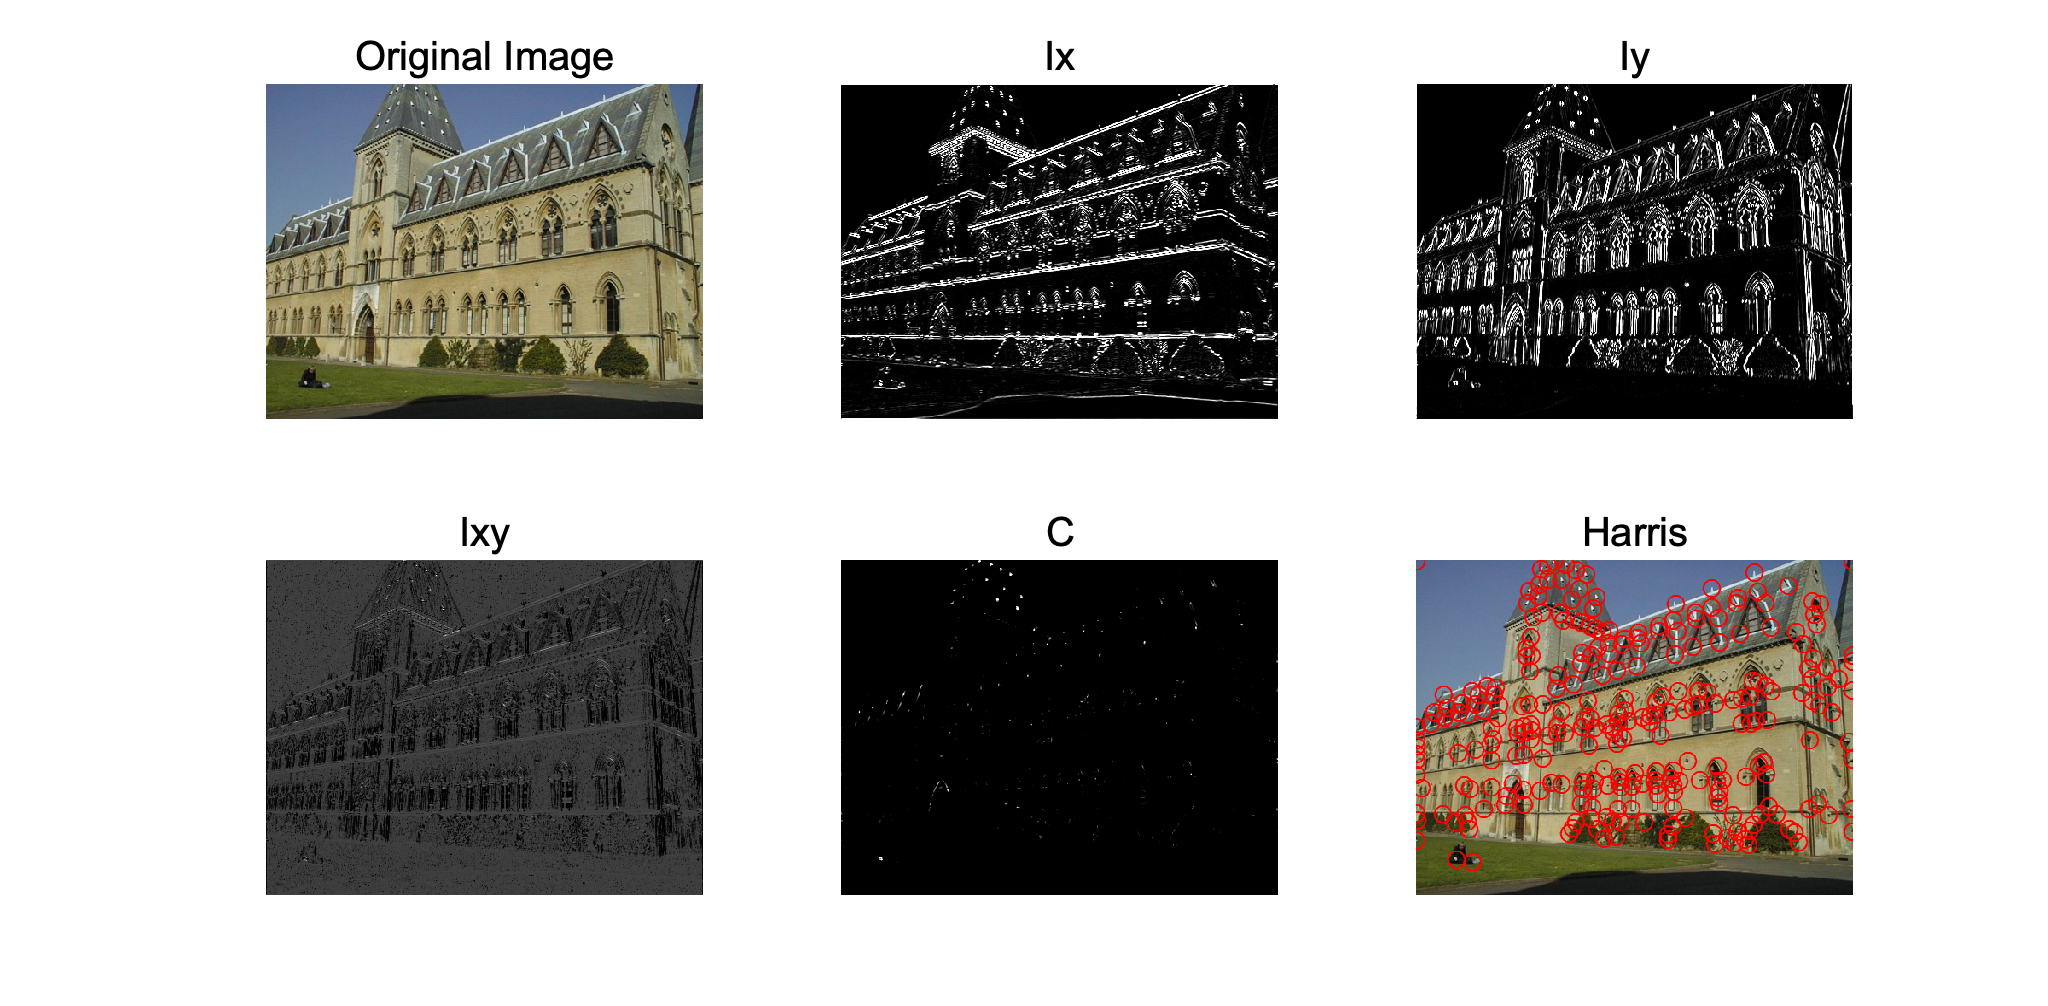
\includegraphics[scale=0.2]{figures/corner3.png}
	}} 
	\caption{Example of Harris corner detection.}
\end{figure*}


\section{RANSAC}
In this exercise, you will work on line fitting using RANSAC. Use the following code to generate simulated data.
\lstinputlisting{ransac.m}
Recall the pipeline of RANSAC:
\begin{enumerate}
\item Randomly select n samples from observations: for $2$D line fitting, we need at least $2$ points, so $n=2$. Useful \textsc{Matlab} functions: \textbf{randperm}. 
\item Model estimation: here we need to estimate the line parameters. Recall estimating a line from two points with homogeneous coordinates which you have already done in the first assignment.
\item Compute Consensus: apply a model-specific loss function to each observation and the model obtained, the response could serve as the consensus. So here we can use the point-to-line distance as the  model-specific loss function. The distance obtained is the consensus.
\item Classifier inliers and outliers using a predefined threshold. You can try with different threshold. Save the model with the largest number of iniliers.
\item Iterate.
\end{enumerate}
Result expected:
\begin{figure*}[thpb]
	\setlength{\fboxrule}{0.0pt}      
	\framebox{\parbox{6.5in}{
			\centering
			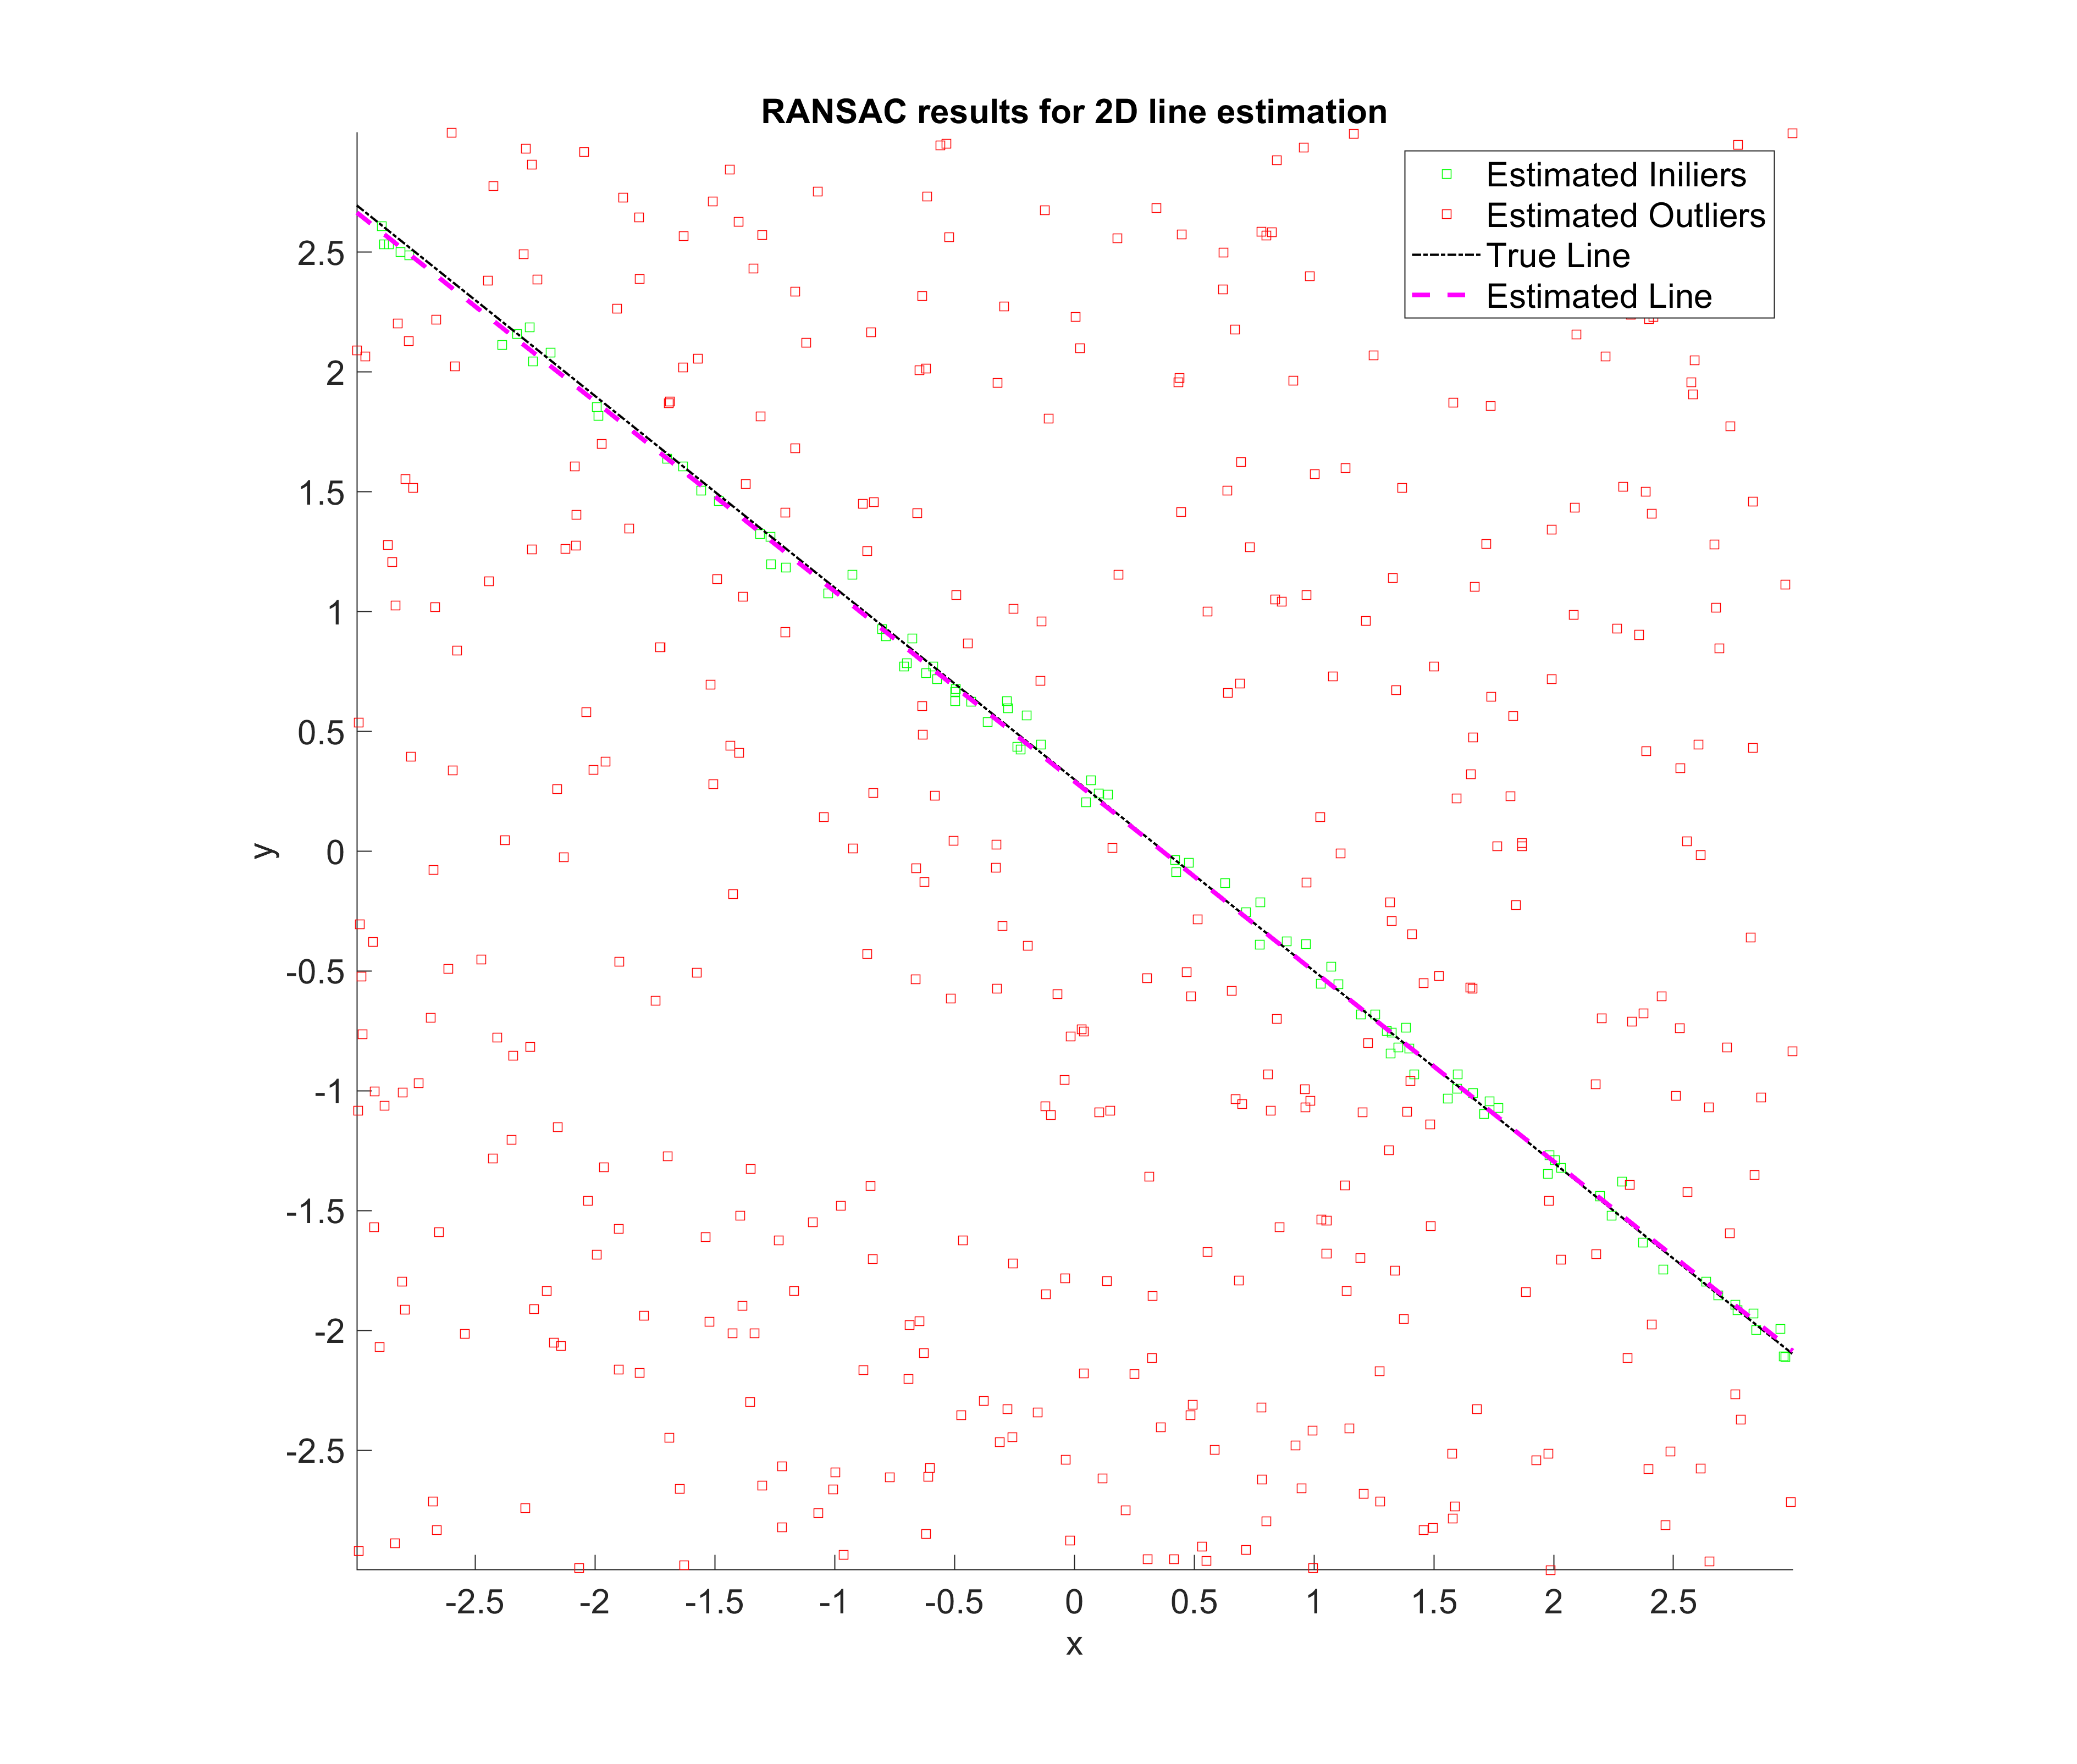
\includegraphics[scale=0.5]{figures/ransac.png}
	}} 
	\caption{Example of RANSAC line fitting.}
\end{figure*}

\bibliography{hand_eye_calibration} 
\bibliographystyle{ieeetr}

\end{document}